% Authored results moved from the application fiche; shared with its standalone.



We can find in \cref{fig:spec:app-feelpp:hl-31:results:visualization-solution} some
examples of 3D visualization that represent fields obtained by solving the
thermoelectric problem. We have the temperature solution and other quantities
evaluated at \textbf{PostProcess} phase such as current density, electric
potential, and electric fields.

The performance analysis has been in the Gaya cluster.
We have run the benchmark with discretizations P1 and P2.
About the \Feelpp distribution, we use native Ubuntu Jammy packages in Gaya.
The results on these machines are illustrated in
\cref{fig:spec:app-feelpp:hl-31:results:performance_times_M1_gaya} %,fig:feelpp:spec:hl-31:results:performance_times_M1_discoverer
respectively. The measures presented are the time-consuming of simulation
components related to WP1, namely \textbf{Init}, \textbf{Solve}, and
\textbf{PostProcess}.

In each case analyzed, we have very good scalability, in the sense that we
reduced significantly the execution time by increasing the number of tasks. The
\textbf{Init} phase is the most time-consuming, with a limit quite high compared
to others. This part contains the mesh reading from the disk, which can explain
some bumps sometimes when require many HPC resources.

To conclude, we can say that we successfully ran this benchmark case, and we are
ready to go up to larger problems and more complex modeling.



\begin{figure}[!ht]
  \centering
  \begin{subfigure}[c]{0.49\textwidth}
    \centering
    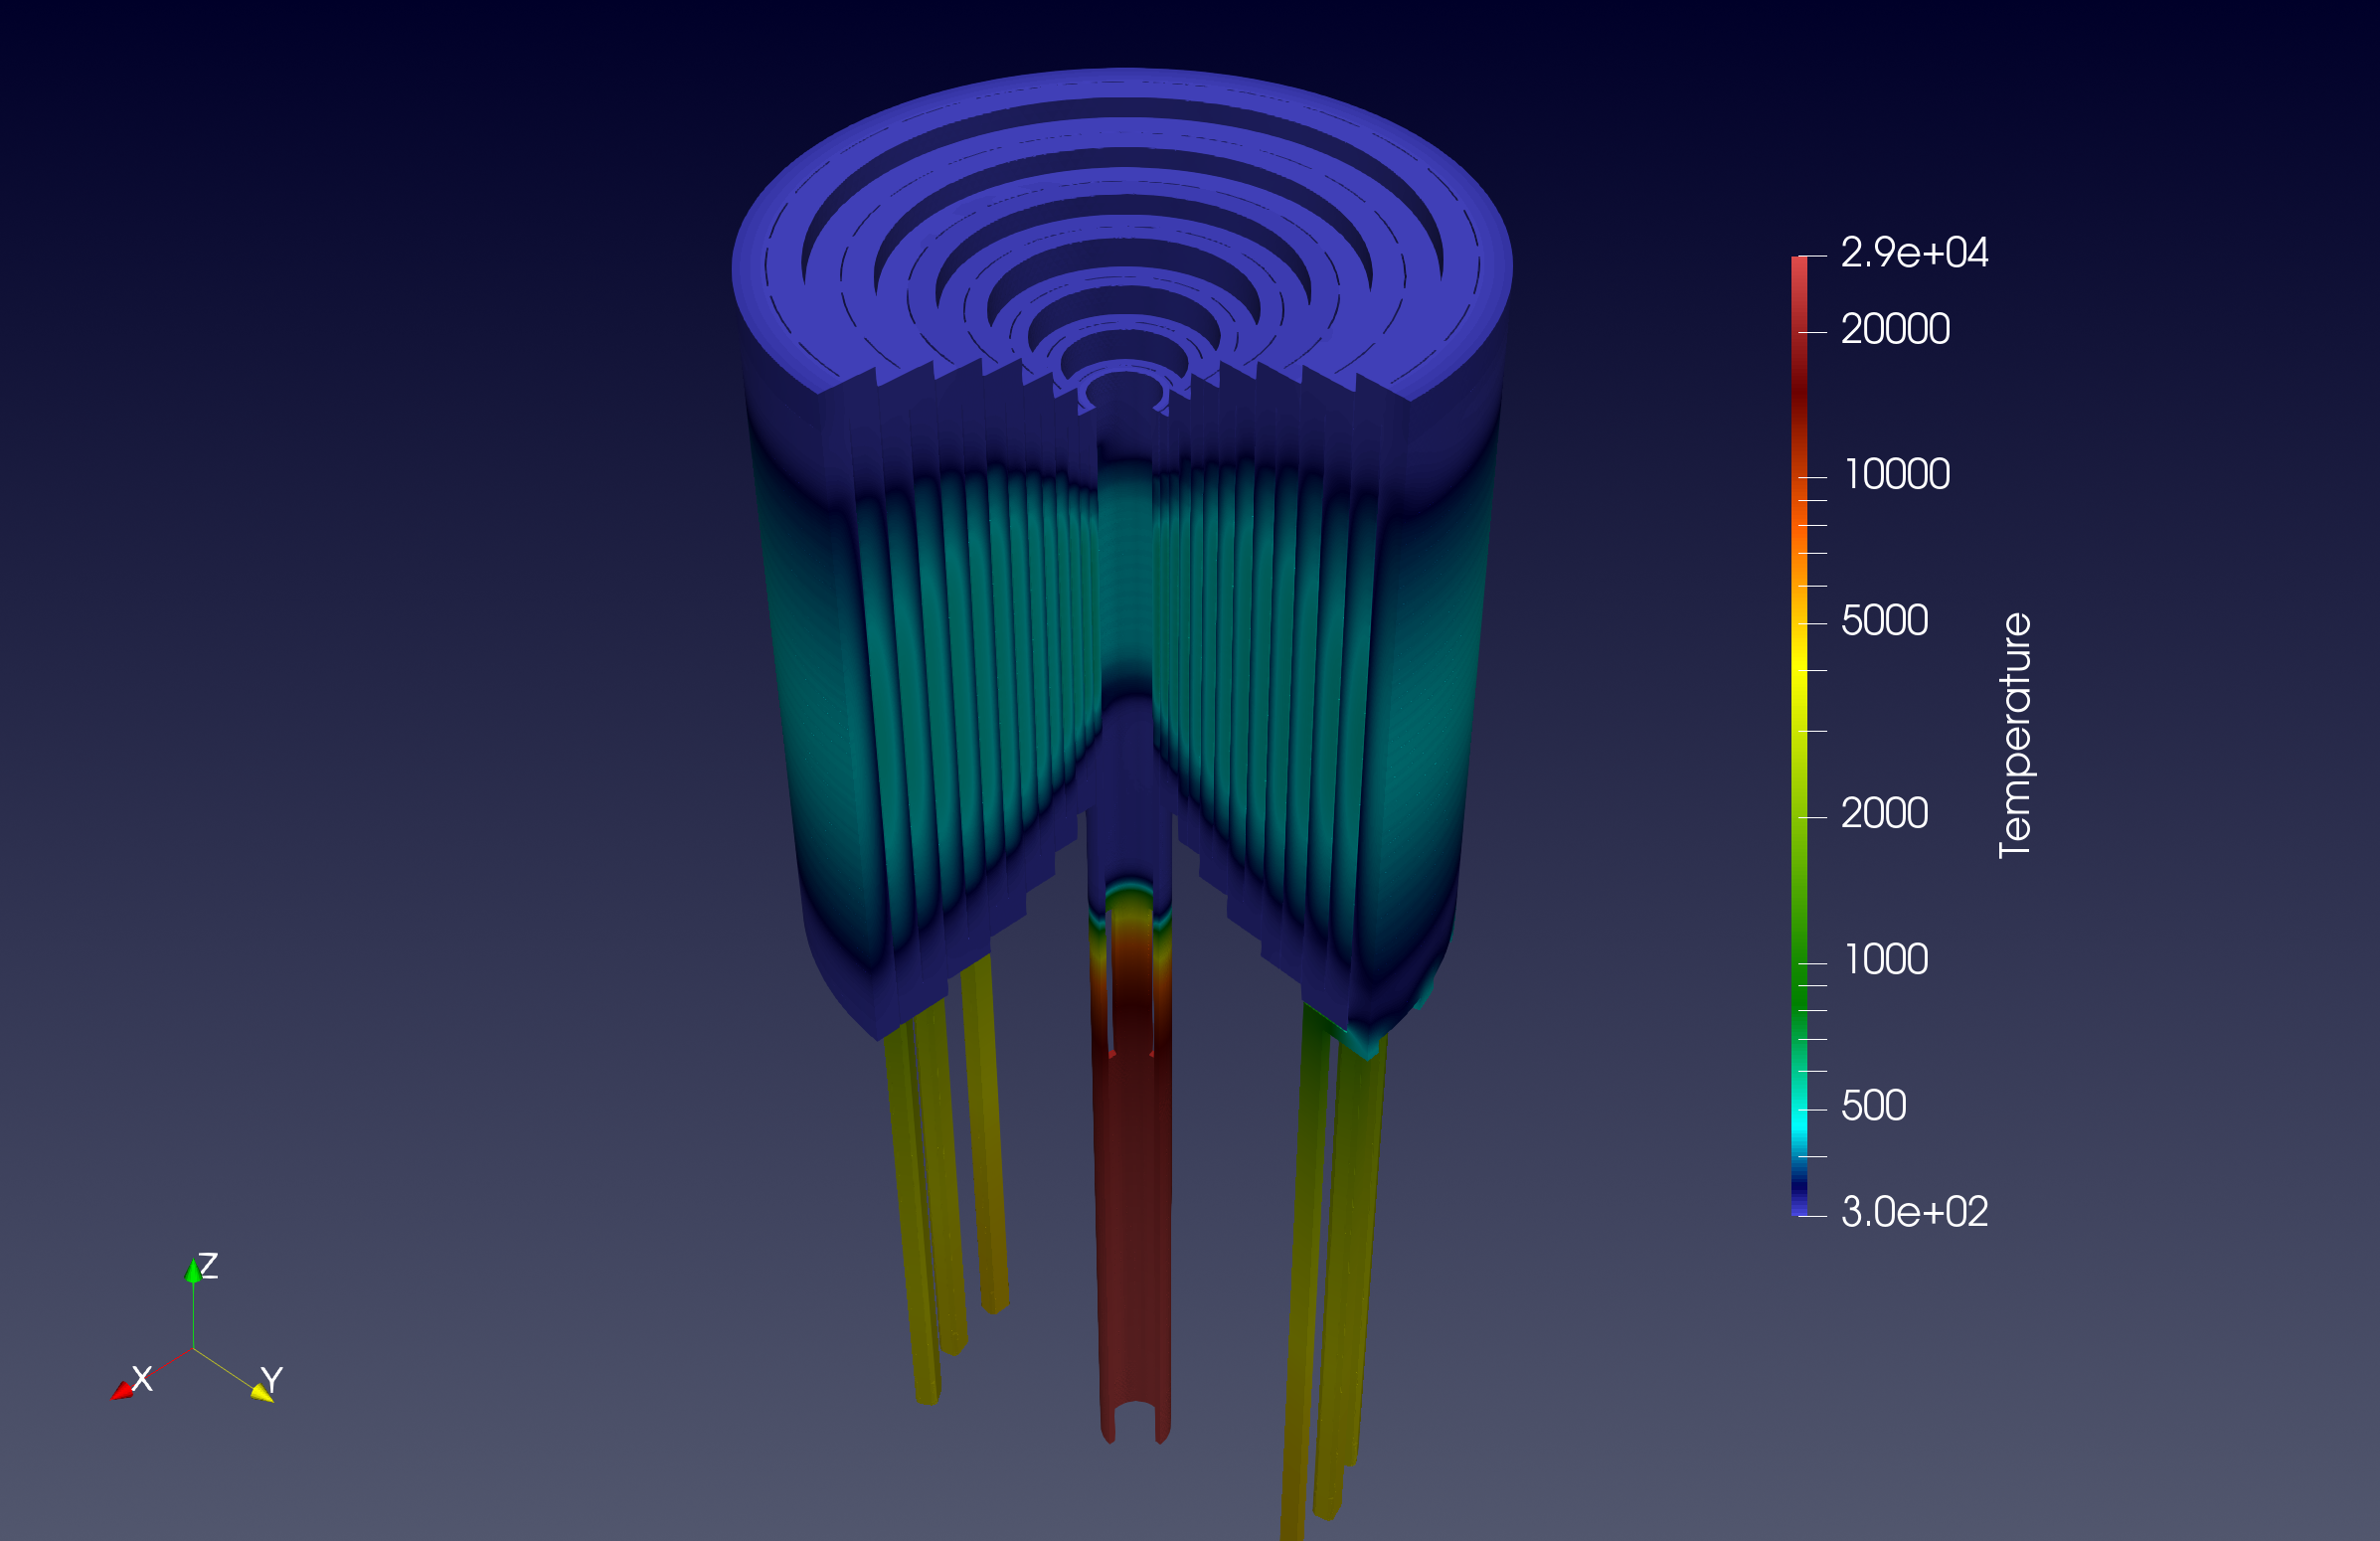
\includegraphics[width=\textwidth]{graphics/feelpp/feelpp-benchmark-HL-31-temperature.png}
    \caption{Temperature}
  \end{subfigure}
  \hfill
  \begin{subfigure}[c]{0.49\textwidth}
    \centering
    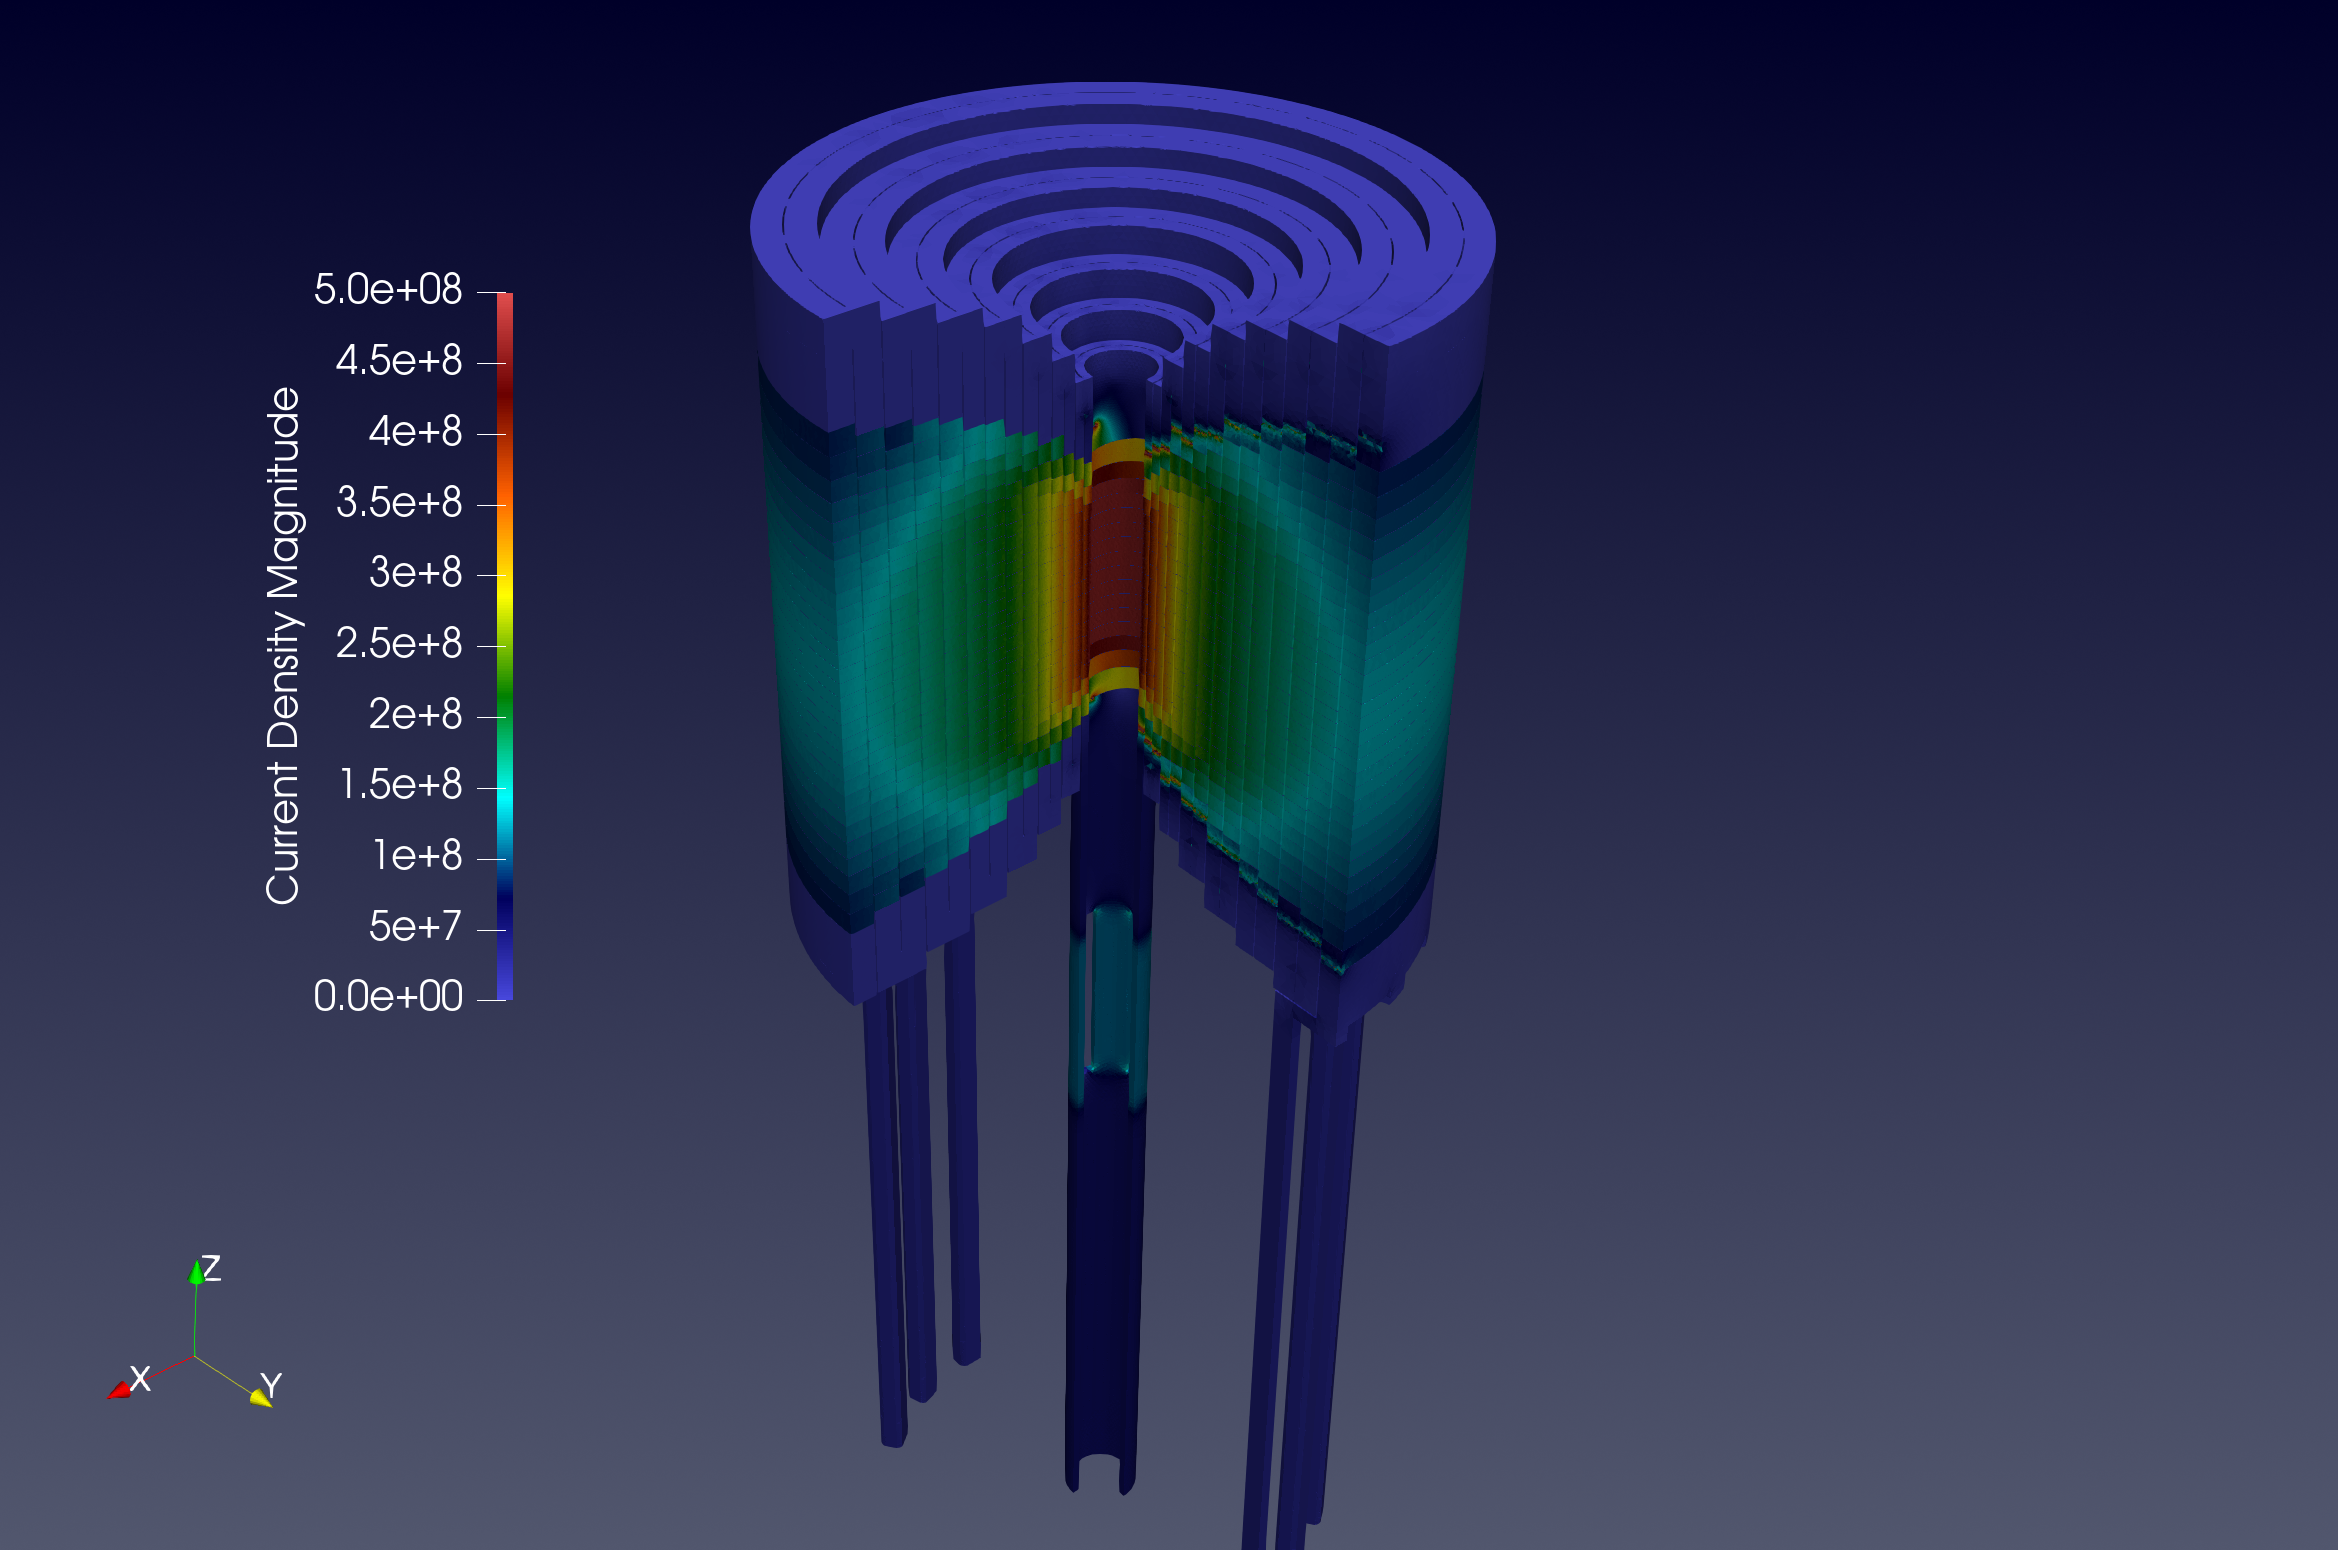
\includegraphics[width=\textwidth]{graphics/feelpp/feelpp-benchmark-HL-31-current_density.png}
    \caption{Current density}
  \end{subfigure}
  \begin{subfigure}[c]{0.49\textwidth}
    \centering
    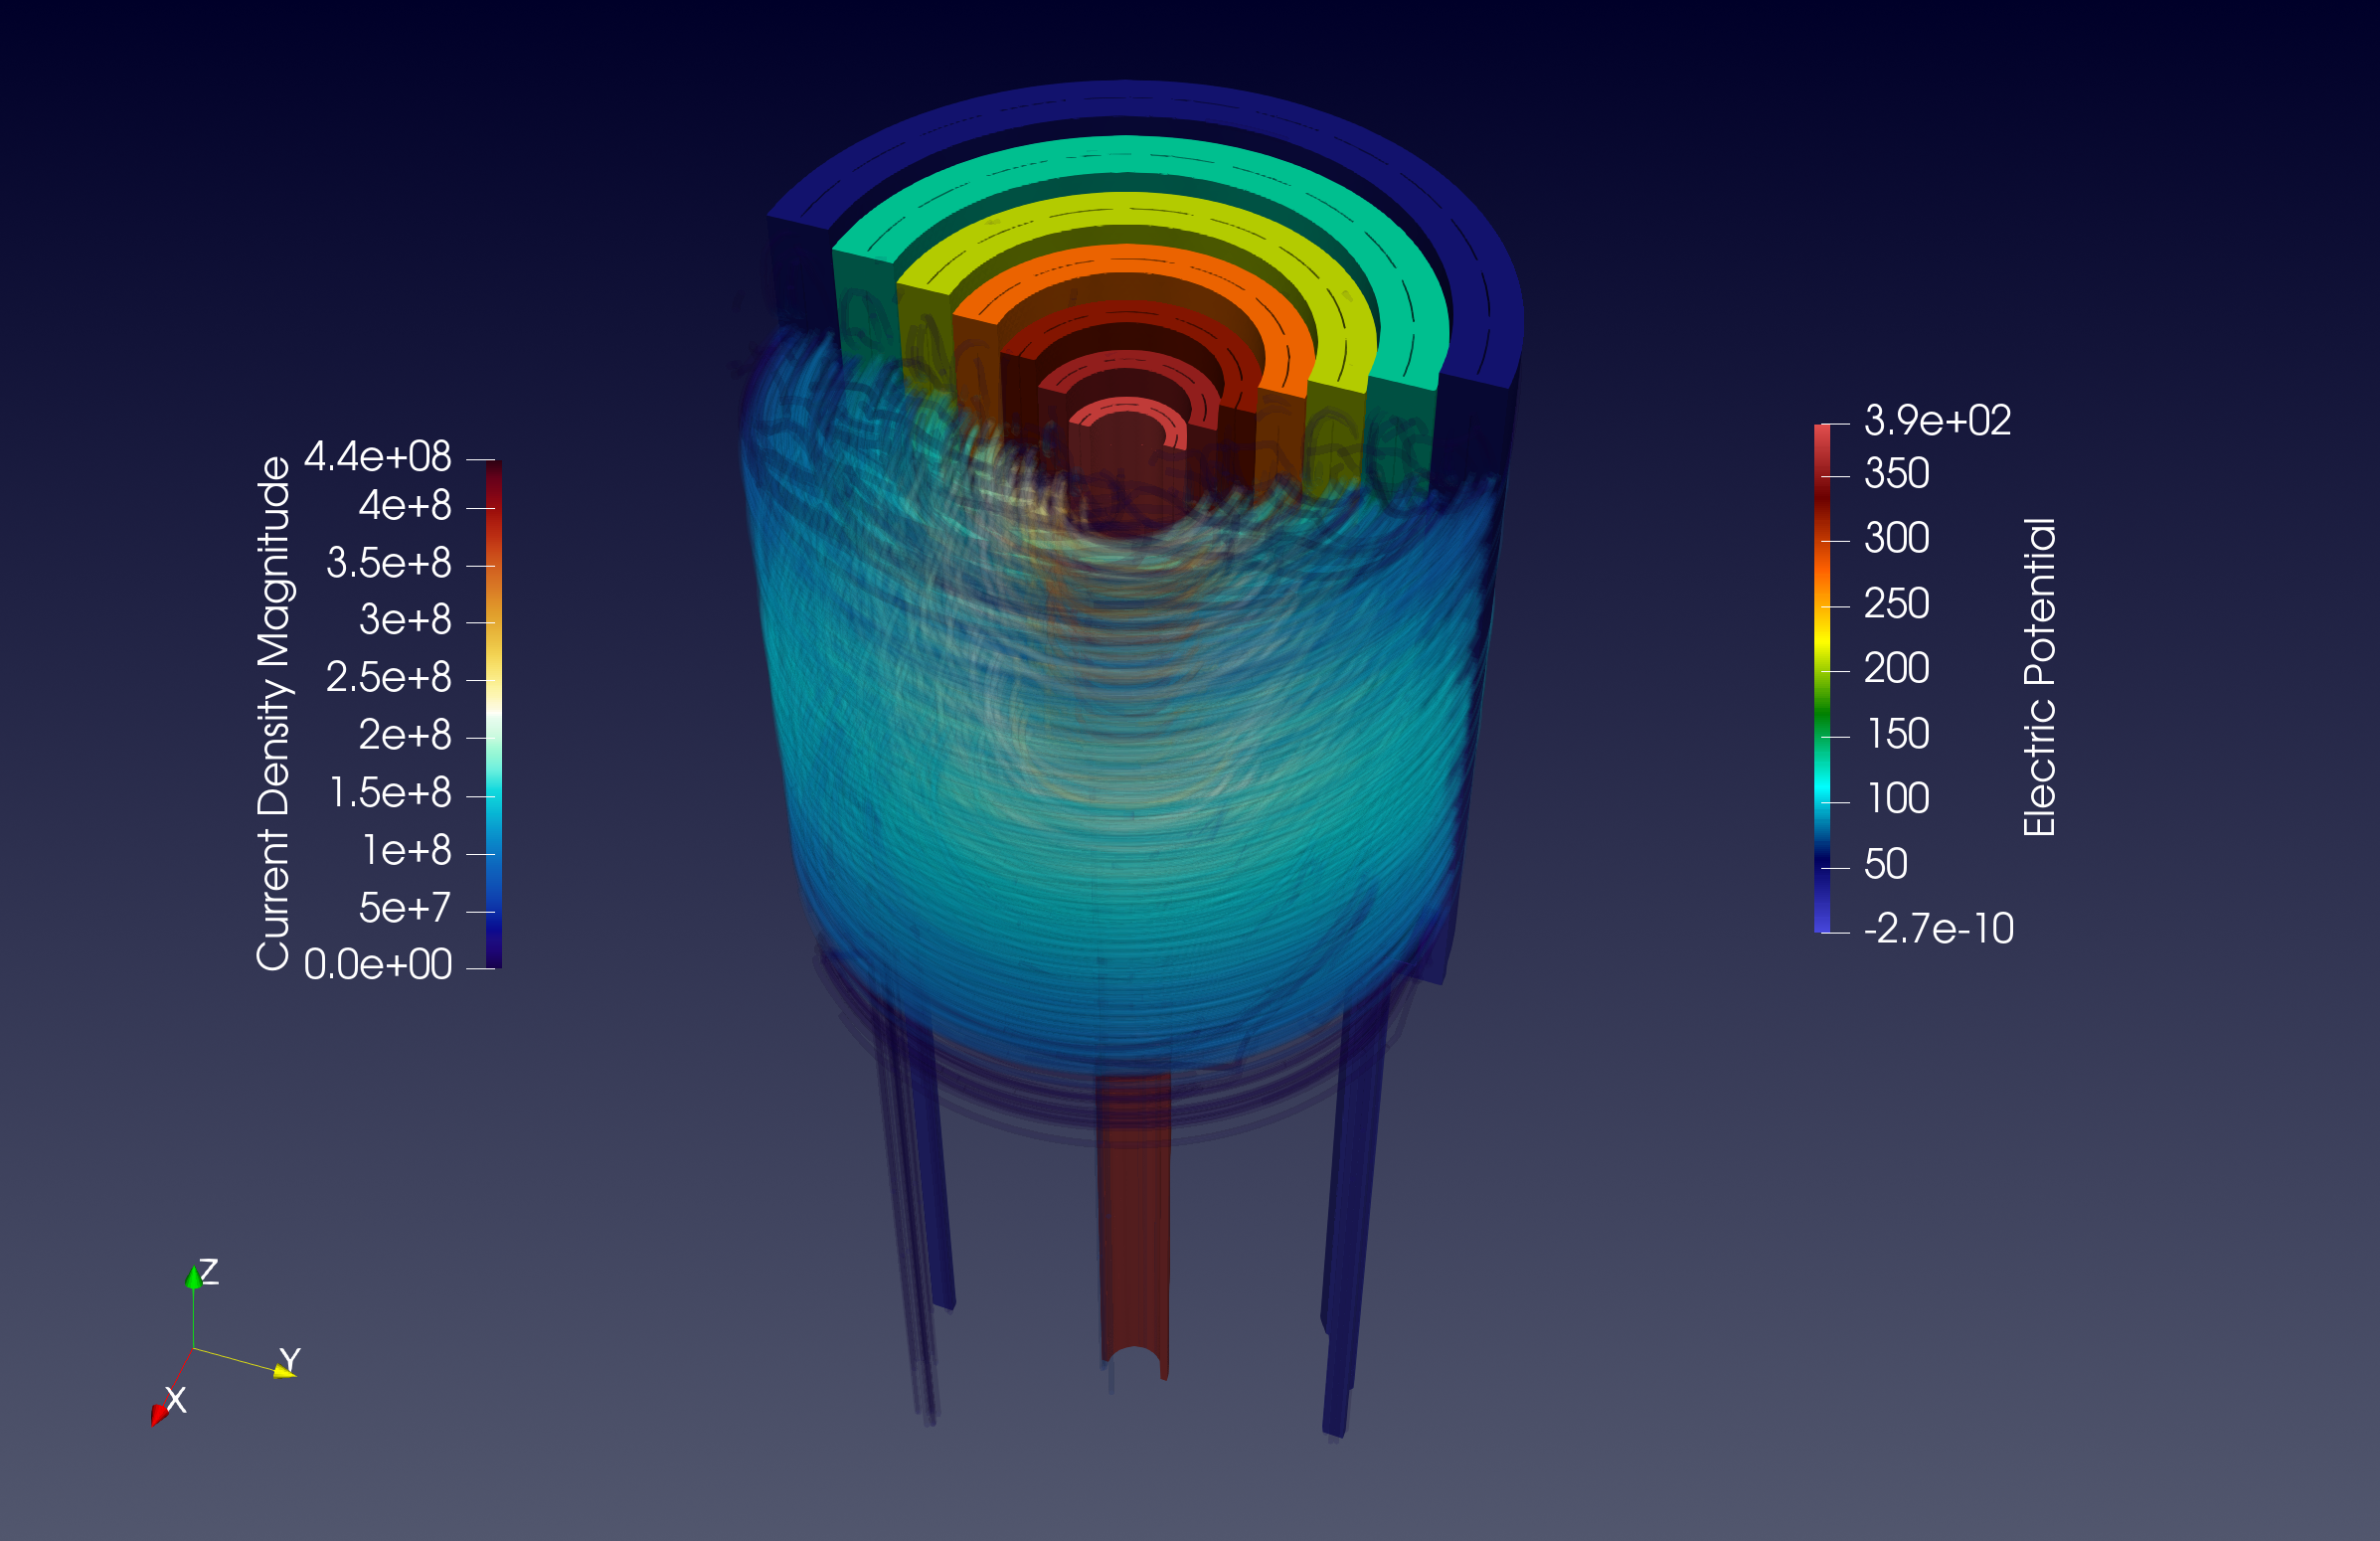
\includegraphics[width=\textwidth]{graphics/feelpp/feelpp-benchmark-HL-31-potential_density_streamines.png}
    \caption{Electric potential and current density on streamlines of electric field}
  \end{subfigure}
  \hfill
  \begin{subfigure}[c]{0.49\textwidth}
    \centering
    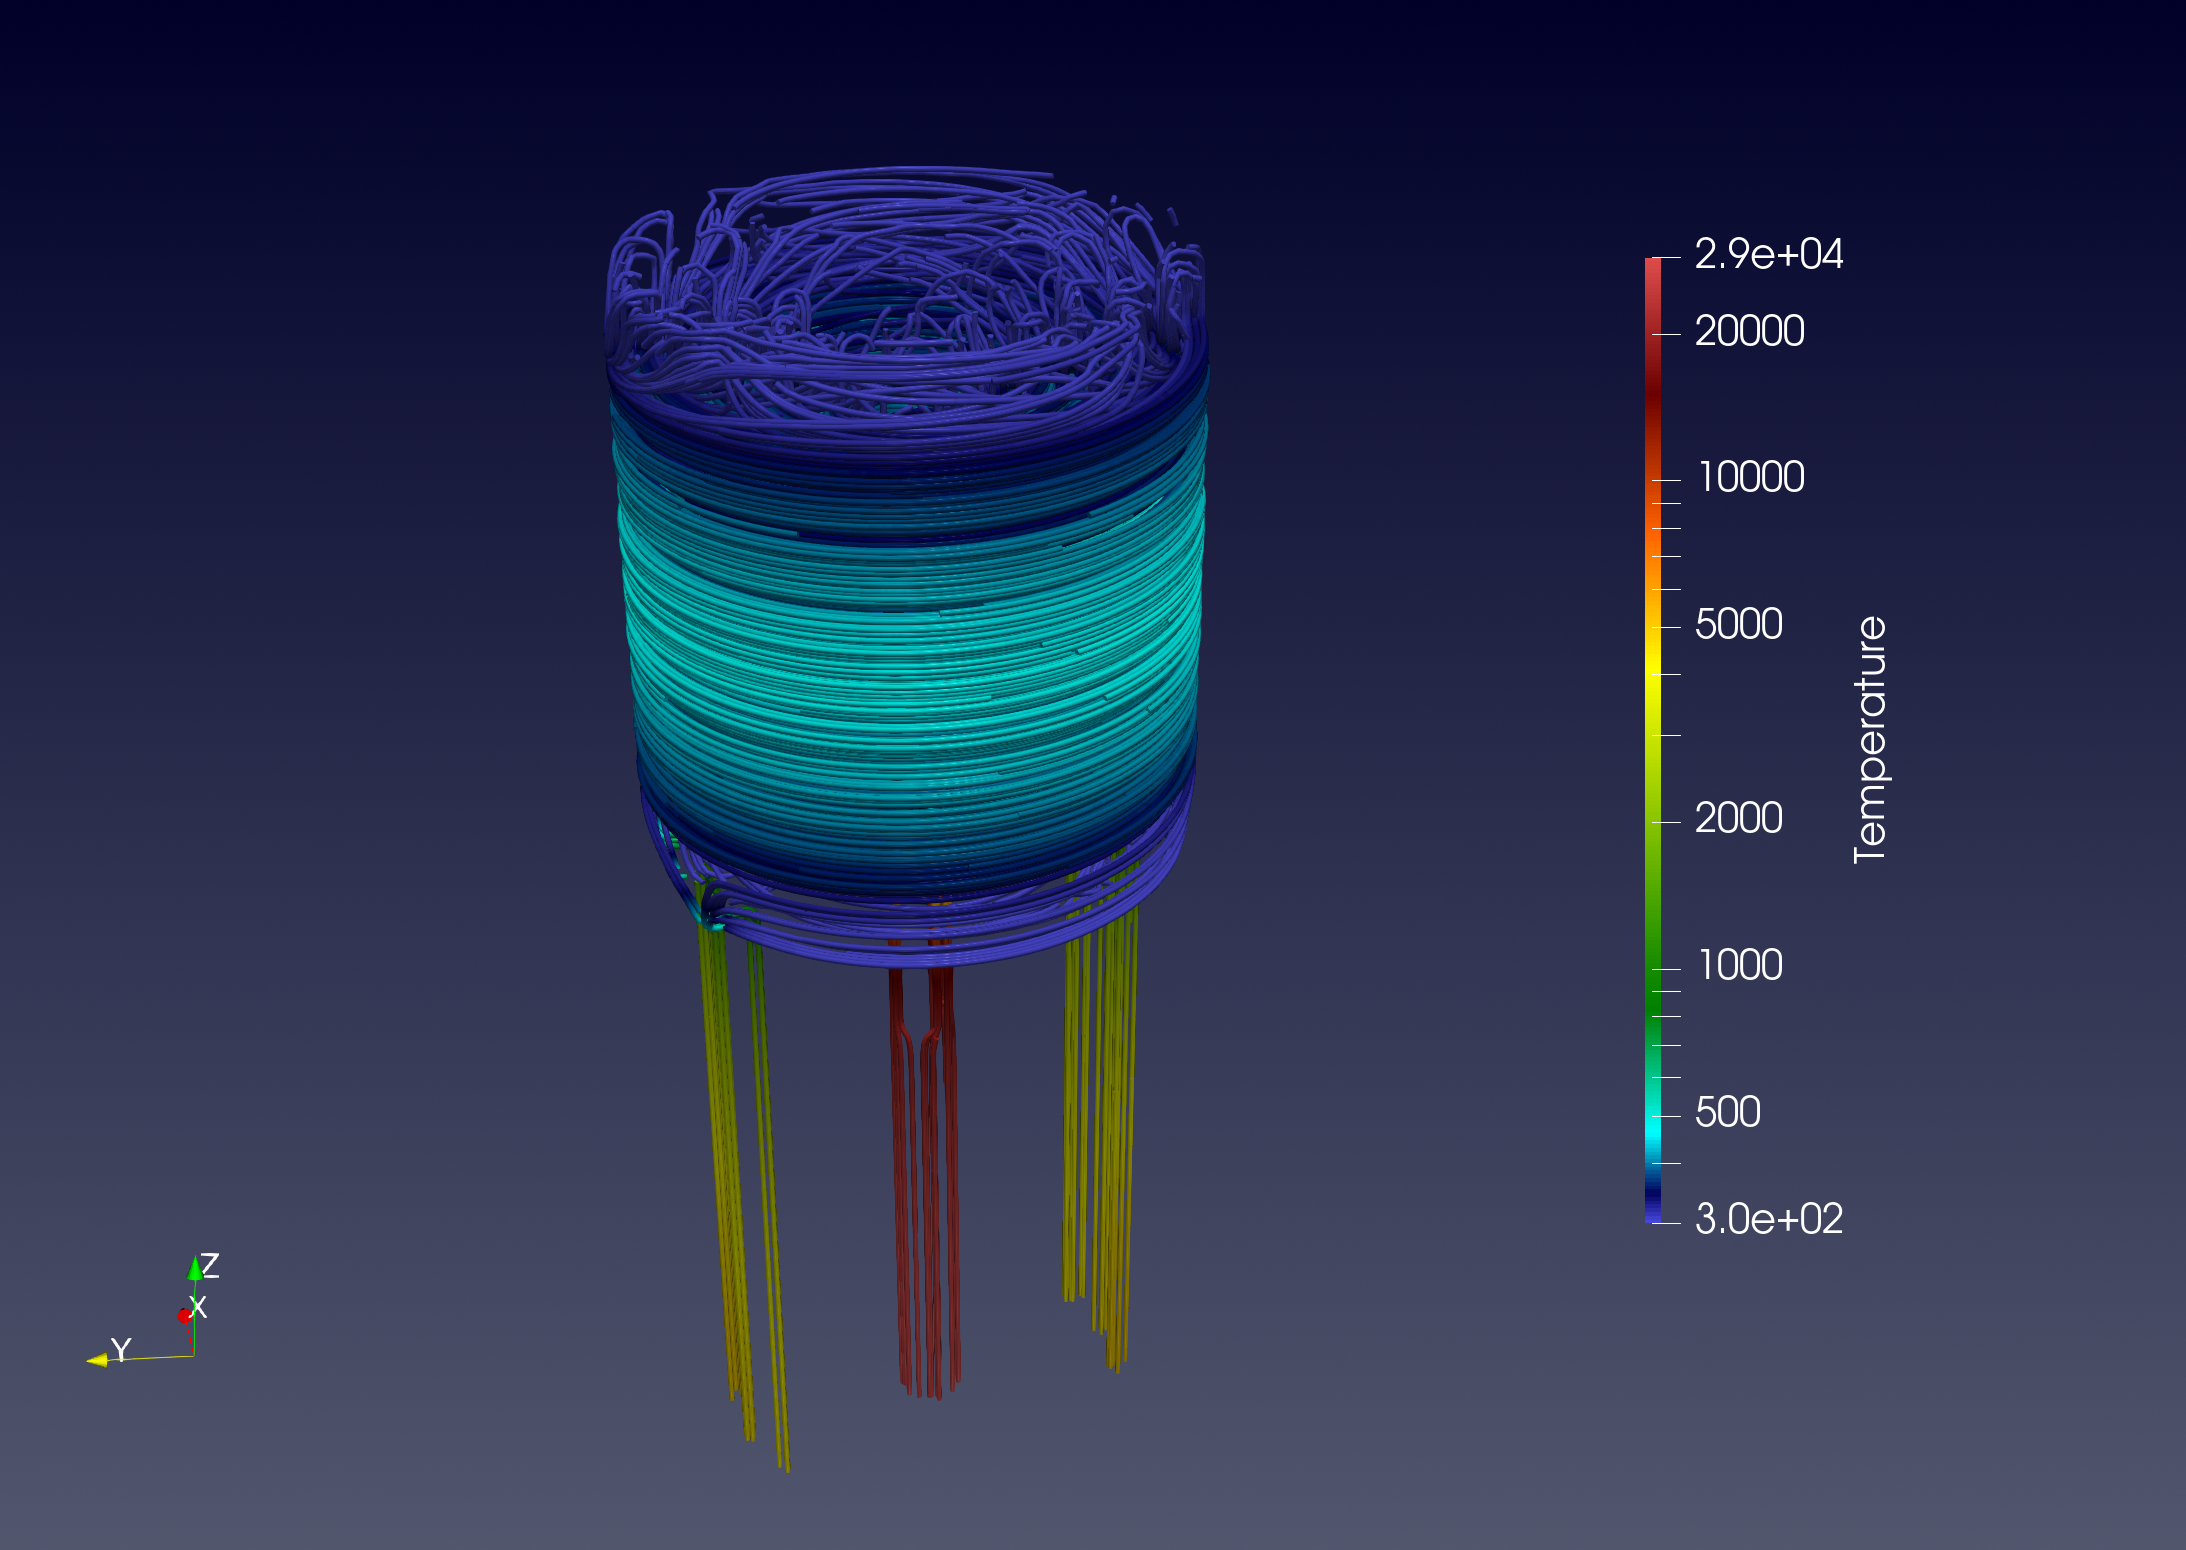
\includegraphics[width=\textwidth]{graphics/feelpp/feelpp-benchmark-HL-31-temperature-streamlines.png}
    \caption{Temperature on streamlines of electric field}
  \end{subfigure}
  \caption{HL-31 benchmarks - solutions}
  \label{fig:spec:app-feelpp:hl-31:results:visualization-solution}
\end{figure}


\foreach [expand list=true] \supercomputerFile/\supercomputerName in {gaya/Gaya} { %,discoverer/Discoverer

  \pgfplotstableread[col sep=comma]{chapters/applications/specs/data/app-feelpp-thermoelectric/exec_times_P1_\supercomputerFile.csv}\dataPa
  \pgfplotstableread[col sep=comma]{chapters/applications/specs/data/app-feelpp-thermoelectric/exec_times_P2_\supercomputerFile.csv}\dataPb
  \pgfplotstableread[col sep=comma]{chapters/applications/specs/data/app-feelpp-thermoelectric/speedup_P1_\supercomputerFile.csv}\dataSpeedupPa
  \pgfplotstableread[col sep=comma]{chapters/applications/specs/data/app-feelpp-thermoelectric/speedup_P2_\supercomputerFile.csv}\dataSpeedupPb

  \begin{figure}[!ht]
    \centering

    \def\chartBarPlot##1##2{
      \barChart[ybar, width=0.97\textwidth, height=0.6172\textwidth,
      xticklabels from table={##2}{tasks},
      x tick label style={ rotate=-45 },
      ylabel={Execution Time (s)},
      legend style={at={(0.5,1.02)}, anchor=south,font=\tiny,legend columns=-1}
      ]{
        {table=##1,column=Init,legend=Init,color=customdarkblue},
        {table=##1,column={Create Mesh},legend={Create Mesh},color=custompurple},
        {table=##1,column=Solve,legend=Solve,color=customcyan},
        {table=##1,column=Export,legend=PostProcess,color=customorange}
      }
    }

    \def\speedupPlot##1##2{
      \begin{tikzpicture}
        \begin{axis}[
          width=0.97\textwidth, height=0.6172\textwidth,
          ymin=0,
          xlabel={Tasks},
          ylabel={Speedup},
          xtick=data,
          xticklabels from table={##2}{tasks},
          x tick label style={ rotate=-45 },
          xticklabel style={font=\small},
          yticklabel style={font=\small},
          ymajorgrids=true, grid style={dashed, gray!40},
          legend style={at={(0.5,1.02)}, anchor=south, font=\tiny, legend columns=3}
        ]
          % Plot optimal and half-optimal bounds
          \addplot[thick, dashed, color=black] table [x expr=\coordindex, y=optimal] {##2};
          \addlegendentry{Optimal}

          \addplot[thick, dotted, color=black] table [x expr=\coordindex, y=half-optimal] {##2};
          \addlegendentry{Half-optimal}

          % Plot actual speedup
          \addplot[thick, mark=*, mark size=1.5pt, color=customdarkblue] table [x expr=\coordindex, y=Init] {##2};
          \addlegendentry{Init}

          \addplot[thick, mark=square*, mark size=1.5pt, color=custompurple] table [x expr=\coordindex, y={Create Mesh}] {##2};
          \addlegendentry{Create Mesh}

          \addplot[thick, mark=triangle*, mark size=1.5pt, color=customcyan] table [x expr=\coordindex, y=Solve] {##2};
          \addlegendentry{Solve}

          \addplot[thick, mark=diamond*, mark size=1.5pt, color=customorange] table [x expr=\coordindex, y=Export] {##2};
          \addlegendentry{PostProcess}
        \end{axis}
      \end{tikzpicture}
    }

    \begin{subfigure}[c]{0.49\textwidth}
      \centering
      \chartBarPlot{dataPa}{\dataPa}
      \caption{\texttt{M1} - \texttt{$P_1$} (Execution Time)}
    \end{subfigure}
    \hfill
    \begin{subfigure}[c]{0.49\textwidth}
      \centering
      \speedupPlot{dataSpeedupPa}{\dataSpeedupPa}
      \caption{\texttt{M1} - \texttt{$P_1$} (Speedup)}
    \end{subfigure}

    \vspace*{0.04\textwidth}

    \begin{subfigure}[c]{0.49\textwidth}
      \centering
      \chartBarPlot{dataPb}{\dataPb}
      \caption{\texttt{M1} - \texttt{$P_2$} (Execution Time)}
    \end{subfigure}
    \hfill
    \begin{subfigure}[c]{0.49\textwidth}
      \centering
      \speedupPlot{dataSpeedupPb}{\dataSpeedupPb}
      \caption{\texttt{M1} - \texttt{$P_2$} (Speedup)}
    \end{subfigure}

    \caption{HL-31 benchmarks - Execution time and speedup of main simulation components
      - \supercomputerName \  supercomputer}
    \label{fig:spec:app-feelpp:hl-31:results:performance_times_M1_\supercomputerFile}
  \end{figure}
}


\paragraph{Challenges Identified}

\begin{itemize}
\item HPC experiments with other kinds of discretizations:
  \begin{itemize}
  \item Modelling: nonlinear, Maxwell, ...
  \item HDG method
  \item Geometry complexity
  \end{itemize}
\item Go to extreme HPC scale: Partitioning and IO issues
\end{itemize}
